\documentclass[11pt]{article}
\usepackage[usenames, dvipsnames]{color}
\usepackage[margin=1in,vmargin=1in]{geometry}
\usepackage[utf8]{inputenc}
\usepackage[english]{babel}
\usepackage{tikz}
\usepackage{pgfplots}
\usepackage{fancyhdr}
\pagestyle{fancy}
\usepackage{url}
\usepackage[font=small,labelfont=bf,labelsep=period]{caption}
\usepgfplotslibrary{polar}
\usepgflibrary{shapes.geometric}
\usetikzlibrary{calc}
\pgfplotsset{compat=1.5.1}
\pgfmathdeclarefunction{gauss}{2}{%
  \pgfmathparse{1/(#2*sqrt(2*pi))*exp(-((x-#1)^2)/(2*#2^2))}%
}

\pgfmathdeclarefunction{bivar}{4}{%
  \pfgmathparse{1/(2*pi*#2*#4) * exp(-((x-#1)^2/#2^2 +
    (y-#3)^2/#4^2))/2}%
}
\usetikzlibrary{shadows}
\usepackage{graphicx}
\usepackage{graphics}
\usepackage[mode=buildnew]{standalone}
\usepackage{amsmath}
\usepackage{amsthm}
\usepackage{amssymb}
\usepackage{changepage}
\usepackage{float}
\DeclareMathOperator*{\argmin}{arg\,min}
\newcommand*{\everymodeprime}{\ensuremath{\prime}}
\usepackage [autostyle, english = american]{csquotes}
\usepackage[backend=bibtex,sorting=none]{biblatex}
\usepackage{wrapfig}
\usepackage{csvsimple}
\bibliography{Master}
\graphicspath{ {plots/} {figures/} }
\definecolor{purduegold}{cmyk}{.43,.56,1,0}
\newcommand{\mcolor}[2][red]{{\color{#1}\textbf{#2}}}
\pgfplotsset{compat=1.6}

\title{CS 573: Homework 4}
\author{Kent Gauen}
\date{\today}
\begin{document}
\maketitle


\section*{Problem 1: Do Ensembles Improve Performance?}

\subsection*{(a)}

\begin{minipage}{0.5\textwidth}
\begin{figure}[H]
  \centering
  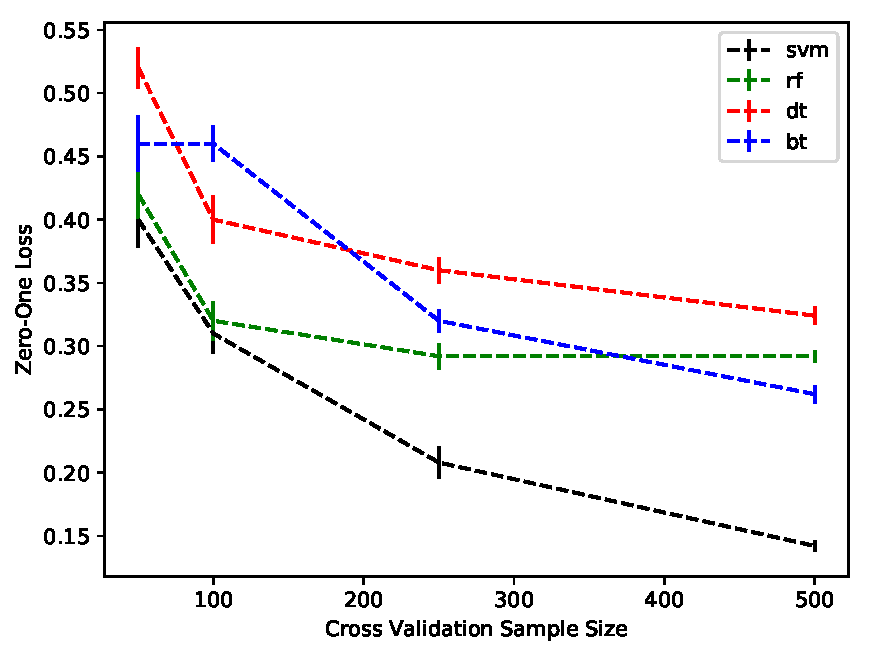
\includegraphics[width=\linewidth]{experiment_1}
  \caption{Learning Curves for three tree models and Support Vector Machine (SVM).}
\end{figure}
\end{minipage}%
\hspace{5mm}
\begin{minipage}{0.5\textwidth}
  Here are comments on the learning curves
\end{minipage}

\subsection*{(b)}

Formulate hypothesis and perform one-tailed t-test

\section*{Problem 2: Do the Number of Features Affect Performance?}

\subsection*{(a)}

\begin{minipage}{0.5\textwidth}
  \begin{figure}[H]
    \centering
    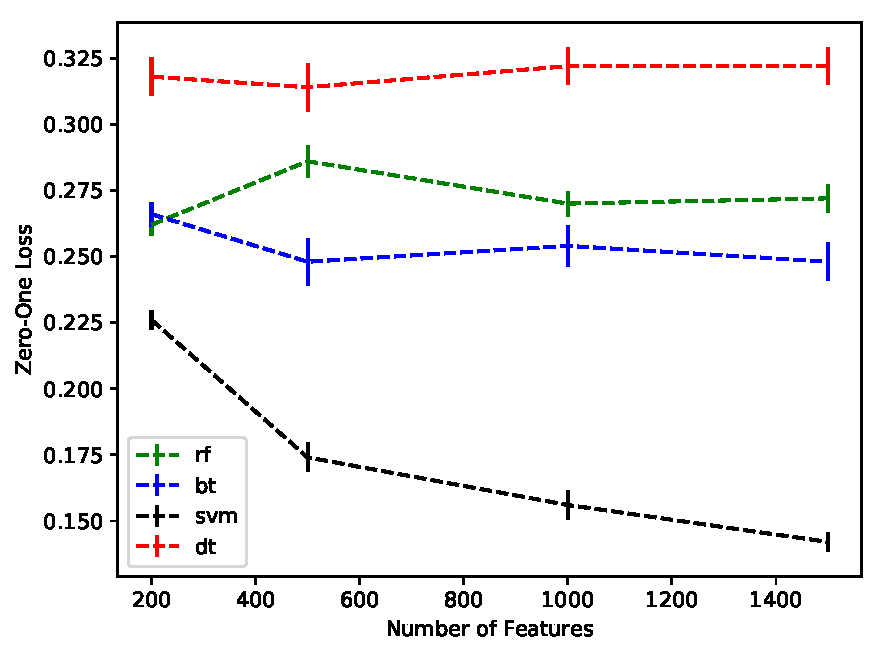
\includegraphics[width=\linewidth]{experiment_2}
    \caption{Learning Curves for three models with three-valued feature values: 0, 1, or 2.}
  \end{figure}
\end{minipage}%
\hspace{5mm}
\begin{minipage}{0.5\textwidth}
  Notice that when compared to Figure 1, the standard error bars are much smaller for each model in this figures. This is related to the fact that the data representation has increased amount of information in the features, which has lead to greater consistancy in performance on the zero-one loss. The consistancy of performance is possibly because of a greater consistancy of information in all samples of cross-validation. Notice how the difference in model performance is less pronounced than with fewer features too. This is likely because of the large model space for each model. Finally, we also note the continued trend down, which went up in Figure 1. The models do not seem to overfit the data, and the error seems to still be trending downward.
\end{minipage}


\subsection*{(b)}

For LR, we predict the zero-one loss would decrease overall as more data is introduced. This is because the data is now encoded with more information, which would imply the model can make a more informative decision. However, with smaller amounts of data it might be challenging for the model to make accurate prediction, because more discrepancies in features might take longer to train. With more complicated features, perhaps the number of samples is larger for the error to start to decrease when the features are non-binary. This is analogous to a ``complex things take more time to learn'' mantra.

\subsection*{(c)}

Our initial hypothesis was correct with respect to our guess the overall error would decrease for LR when the $2$ was introduced into the data. We were also correct that the LR model did not perform as well will the smaller sample size on the three-valued, when compared to the same sample size with binary features.
Another change which we did not predict, is that the standard error smaller for every data sample size. Visually, the difference is significant between Figures 1 and 2. This can be explained by the greater amount of information in the data when the $2$ is added. Therefore even in a small sample, there is a greater opporunity for consistency of information. It seems fair to conclude that samples are less likely to be biased when the feature space grows.




\end{document}